\documentclass{report}
\usepackage[english]{babel}
\usepackage[a4paper,top=2cm,bottom=2cm,left=3cm,right=3cm,marginparwidth=1.75cm]{geometry}

\usepackage{graphicx}
\usepackage{subcaption}
\usepackage[colorlinks=true, allcolors=blue]{hyperref}
\usepackage{minted}
\usepackage{fancyhdr}

\setlength\parindent{0pt}

\fancyfoot{}
\pagestyle{fancy}
\rfoot{By Christopher Ashford}
\cfoot{\thepage}
\title{DRMBM (1994) remake}
\author{Christopher Ashford}
\date{March 2023}

\begin{document}
\maketitle

\tableofcontents

\chapter{Analysis}

\section{Introduction and Background}

Dr Robotnik’s Mean Bean Machine is a 1994 Westernised port of Puyo Puyo for the Sega Genesis/Mega Drive. It is a game that I have enjoyed throughout my childhood on many different forms – cheap emulation consoles, the Sega Mega Drive Collection for Xbox 360, using Fusion emulator on PC among other forms. However, all of these present glaring issues that directly affect the enjoyment of the player – emulation consoles usually are slow with clunky controllers and are not good for much else and thus are not practical to use permanently; the Sega Mega Drive collection on Xbox 360 suffers with a noticeable input lag problem, with inputs sometimes taking hundreds of milliseconds to be processed, directly affecting how fast you can play; PC emulation either results in a small or blurry image and makes it difficult to play with others or share your scores and achievements.

The goal of this project is to solve these problems by creating a superior, native PC remake of the game. Everything in the original game shall work exactly as in the original, including re-constructing the algorithms used for the playstyles of the various AI opponents. I also intend to include many quality of life improvements to solve the problems listed about: multiple customisable input method and handling will be supported, many algorithmic optimisations shall be made to improve performance, graphics shall be upscaled in a way that remains a crisp pixel look instead of introducing blur, an SQL web server will allow score and time leaderboards to exist and a replay file system shall be introduced to allow players to easily share gameplay. This project exists to create a superior version of DRMBM for a new generation to enjoy, as well as offering a way for modern Puyo Puyo players to enjoy the OPP rule set on modern devices.

If the goals above are reached, further extension goals include the introduction of my own custom AI opponents with algorithms designed for optimal, “perfect” gameplay and the use of web sockets to facilitate real-time online matches between two remote players.

\section{Alternative Solutions}

In this section I shall present my research on other Puyo Puyo games, compare the advantages and disadvantages of different versions from the perspective of the end user and take inspiration for my own project.

\subsection{Emulation}

\begin{figure}[ht]
\centering
\begin{subfigure}{0.49\textwidth}
\centering
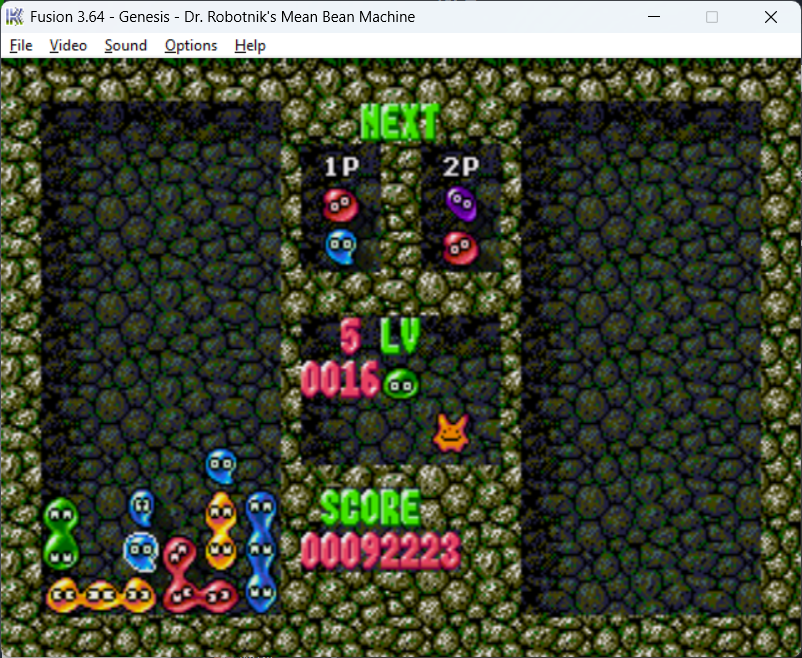
\includegraphics[width = \textwidth]{emulator1.png}
\caption{Fusion emulator}
\label{fig:emu1}
\end{subfigure}
\begin{subfigure}{0.45\textwidth}
\centering
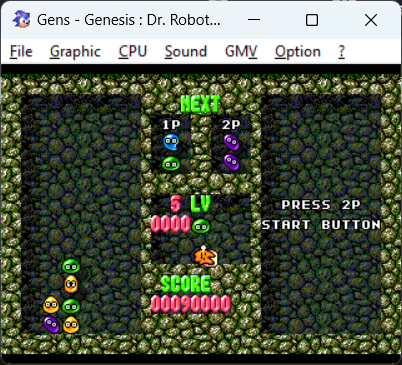
\includegraphics[width = \textwidth]{emulator2.png}
\caption{Gens emulator}
\label{fig:emu2}
\end{subfigure}
\caption{Some examples of emulators running the game}
\label{fig:combined}
\end{figure}

Link: cannot be provided due to specialised hardware being required to dump the ROM. Yet another disadvantage.

Many different emulators exist for the Sega Mega Drive, such as Fusion or Gens shown above, or the official Sega emulator that can be found on Steam. These are programs that accept a binary ROM dump of the original cartridge and attempt to emulate the code.
\vspace{0.3cm}

Advantages:

\begin{itemize}
    \renewcommand\labelitemi{--}
    \item Convenient for mass production and distribution.
    Sega can create one Mega Drive emulator and release an entire of library of games that use the same program
    \item True to the original experience.
    Since you are playing a copy of the original game, you can be sure you are getting an authentic experience
    \item While clunky, save states allow you to save high scores and progress through the story, as well as letting you manipulate sequences of beans
\end{itemize}

Disadvantages: 

\begin{itemize}
    \renewcommand\labelitemi{--}
    \item Resolution is locked at the console’s original and upscaling is blurry and unappealing
    \item Very static and not customisable. It is incredibly difficult to edit a ROM if you wanted to play with, for example, different handling or textures
    \item Saving progress is difficult
    \item Emulators are difficult to run and can easily lag on lighter hardware, running the game at higher levels can struggle on older processors
    \item It is impossible to play with friends remotely (or if it is possible, then it’s too difficult for the average user to achieve)
\end{itemize}

\subsection{B Puyo}

\begin{figure}[ht]
\centering
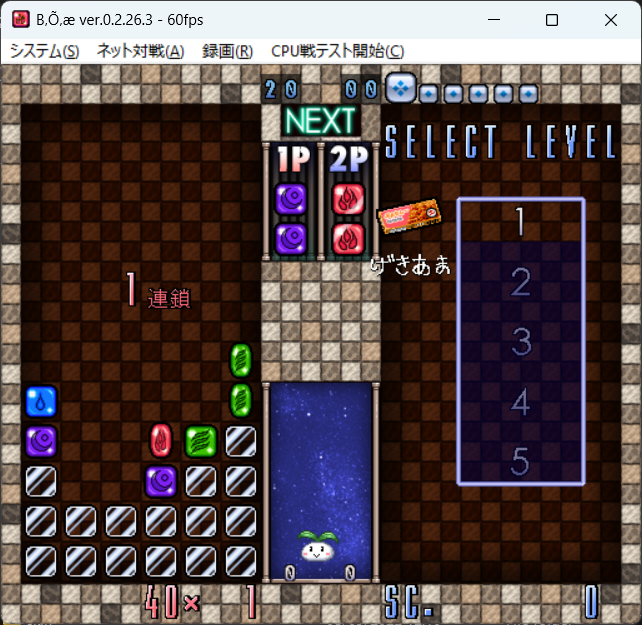
\includegraphics[width=0.3\textwidth]{bpuyo.png}
\caption{\label{fig:bpuyo}A screenshot of B Puyo. Some text is broken running on an English computer.}
\end{figure}
\begin{figure}[ht]
\centering
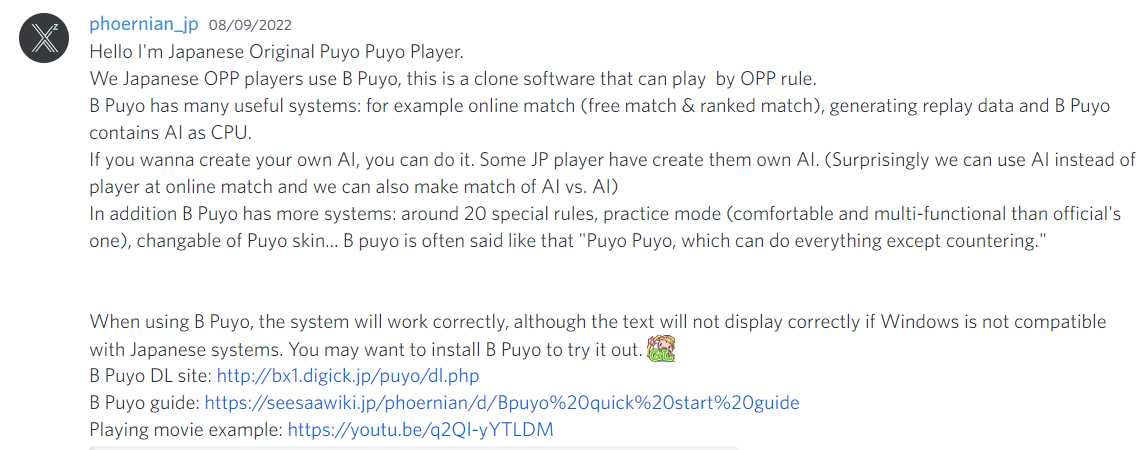
\includegraphics[width=1\textwidth]{discord.png}
\caption{\label{fig:discord}Information about B Puyo from a well known Japanese player.}
\end{figure}
Link: \href{http://bx1.digick.jp/puyo/dl.php}{http://bx1.digick.jp/puyo/dl.php}

B puyo is a popular online Puyo-clone recommended to me by the Japanese community.
\vspace{0.3cm}

Advantages:

\begin{itemize}
    \renewcommand\labelitemi{--}
    \item Custom textures, custom AI, custom rules, custom anything really
    \item Easy to use online multiplayer
    \item Great performance as a native PC program

\end{itemize}

\vspace{3cm}

Disadvantages: 

\begin{itemize}
    \renewcommand\labelitemi{--}
    \item Will only run on Windows, excluding Mac and Linux users
    \item The entire thing is in Japanese, with no translation options. Furthermore, servers are in Japan, creating ping issues for non-Japanese players. This is great for the Japanese community, but unfortunately disadvantages me as a Western player
    \item The resolution is locked to being a small window, making it uncomfortable to use on high-resolution displays
\end{itemize}

\subsubsection{Project GelaVolt}

\begin{figure}[ht]
\centering
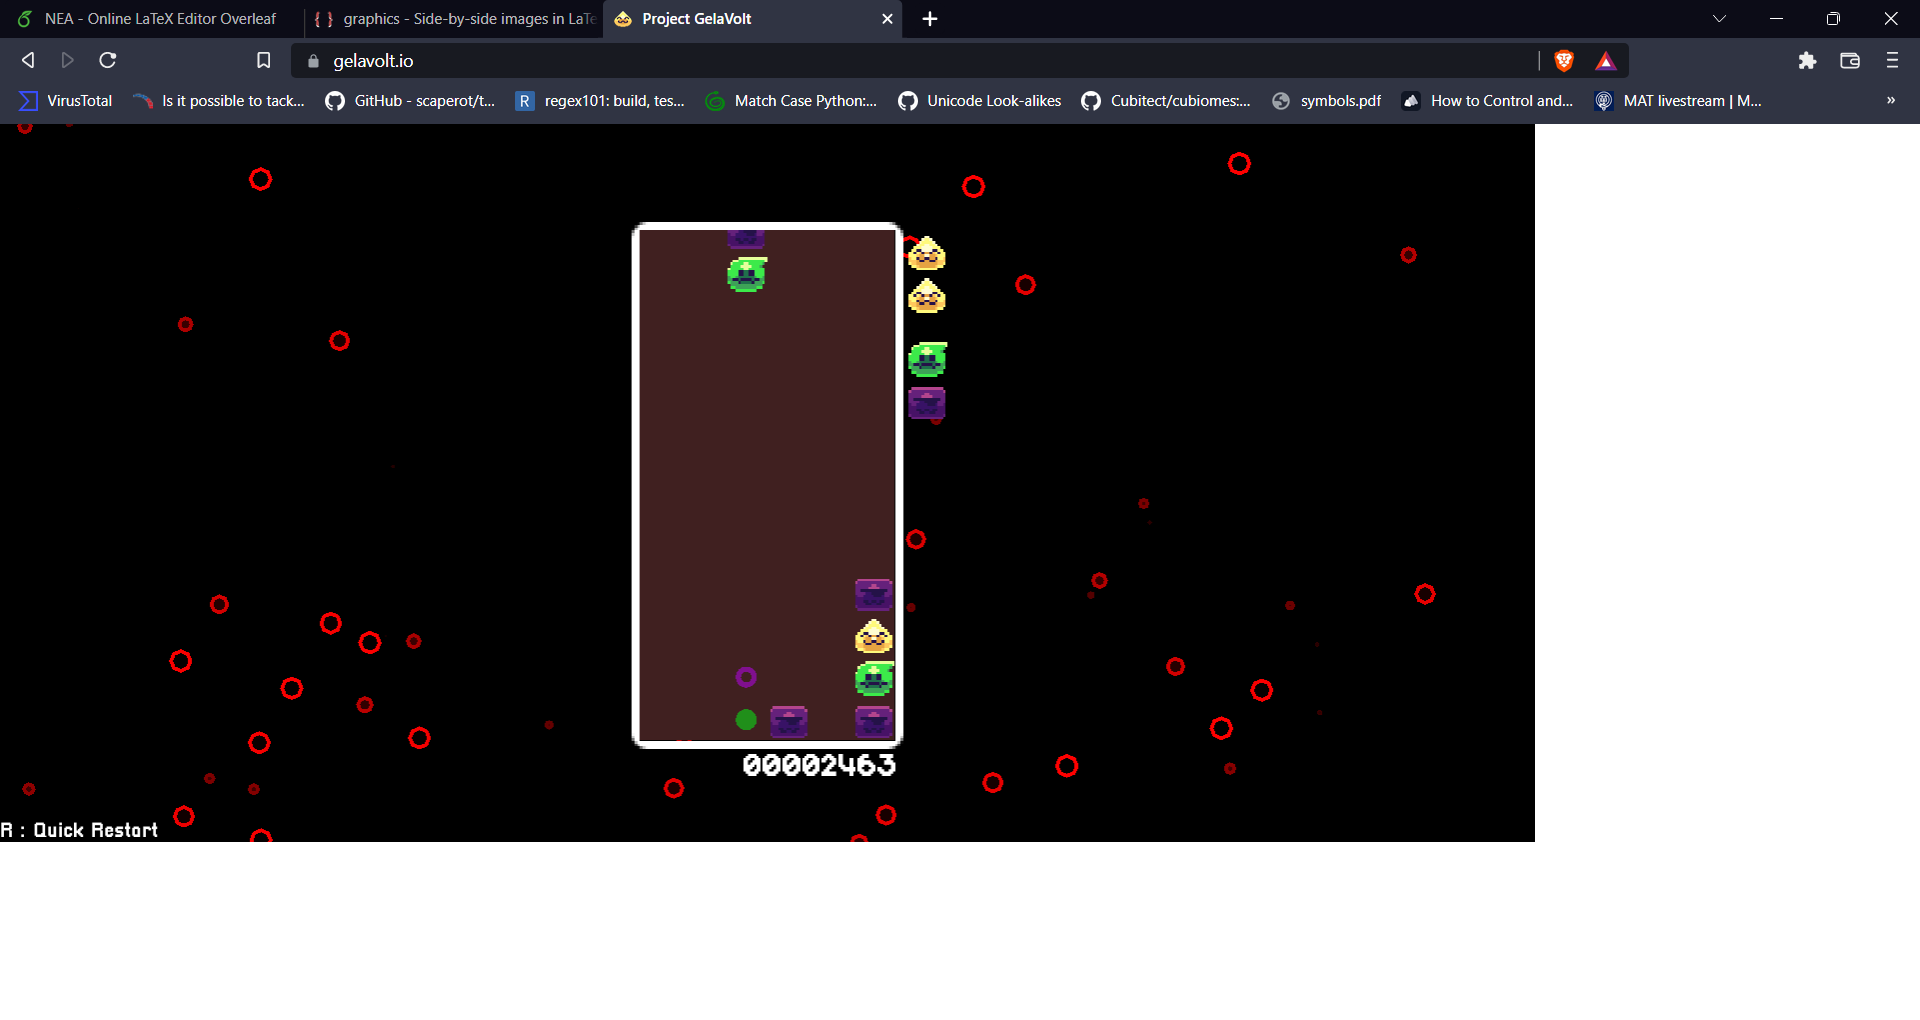
\includegraphics[width=1\textwidth]{gelavolt.png}
\caption{\label{fig:gelavolt}A screenshot of GelaVolt running in a chromium-based web browser.}
\end{figure}
Link: \href{https://gelavolt.io/}{https://gelavolt.io/}

To quote the game’s creator, “Project GelaVolt is a modern, techno-themed pixel art fangame of SEGA's Puyo Puyo series, one of Japan's most successful puzzle fighter franchises. Currently, GelaVolt is focused on the competitive aspects of the game and it's intended purpose is to help introduce people and help people get better at Puyo Puyo. However, if all goes well, GelaVolt will become a free alternative that plans to solve some of the communities problems: lack of players, lack of crossplay and lack of general quality netcode.” It is a Puyo-clone written in Haxe that runs in browsers.
\vspace{0.3cm}

Advantages:

\begin{itemize}
    \renewcommand\labelitemi{--}
    \item Appealing design
    \item Is lightweight and capable of running well in browsers
    \item Supports many different control schemes out of the box (controller, keyboard, etc.)
    \item Only version I’ve played that has hard drop
\end{itemize}

\vspace{0.7cm}

Disadvantages: 

\begin{itemize}
    \renewcommand\labelitemi{--}
    \item Multiplayer is in the works but is currently not supported at the time of writing
    \item Things such as textures are not customisable
    \item Is unstable and crashes regularly
\end{itemize}

\subsection{Puyo Puyo Tetris 2}

\begin{figure}[ht]
\centering
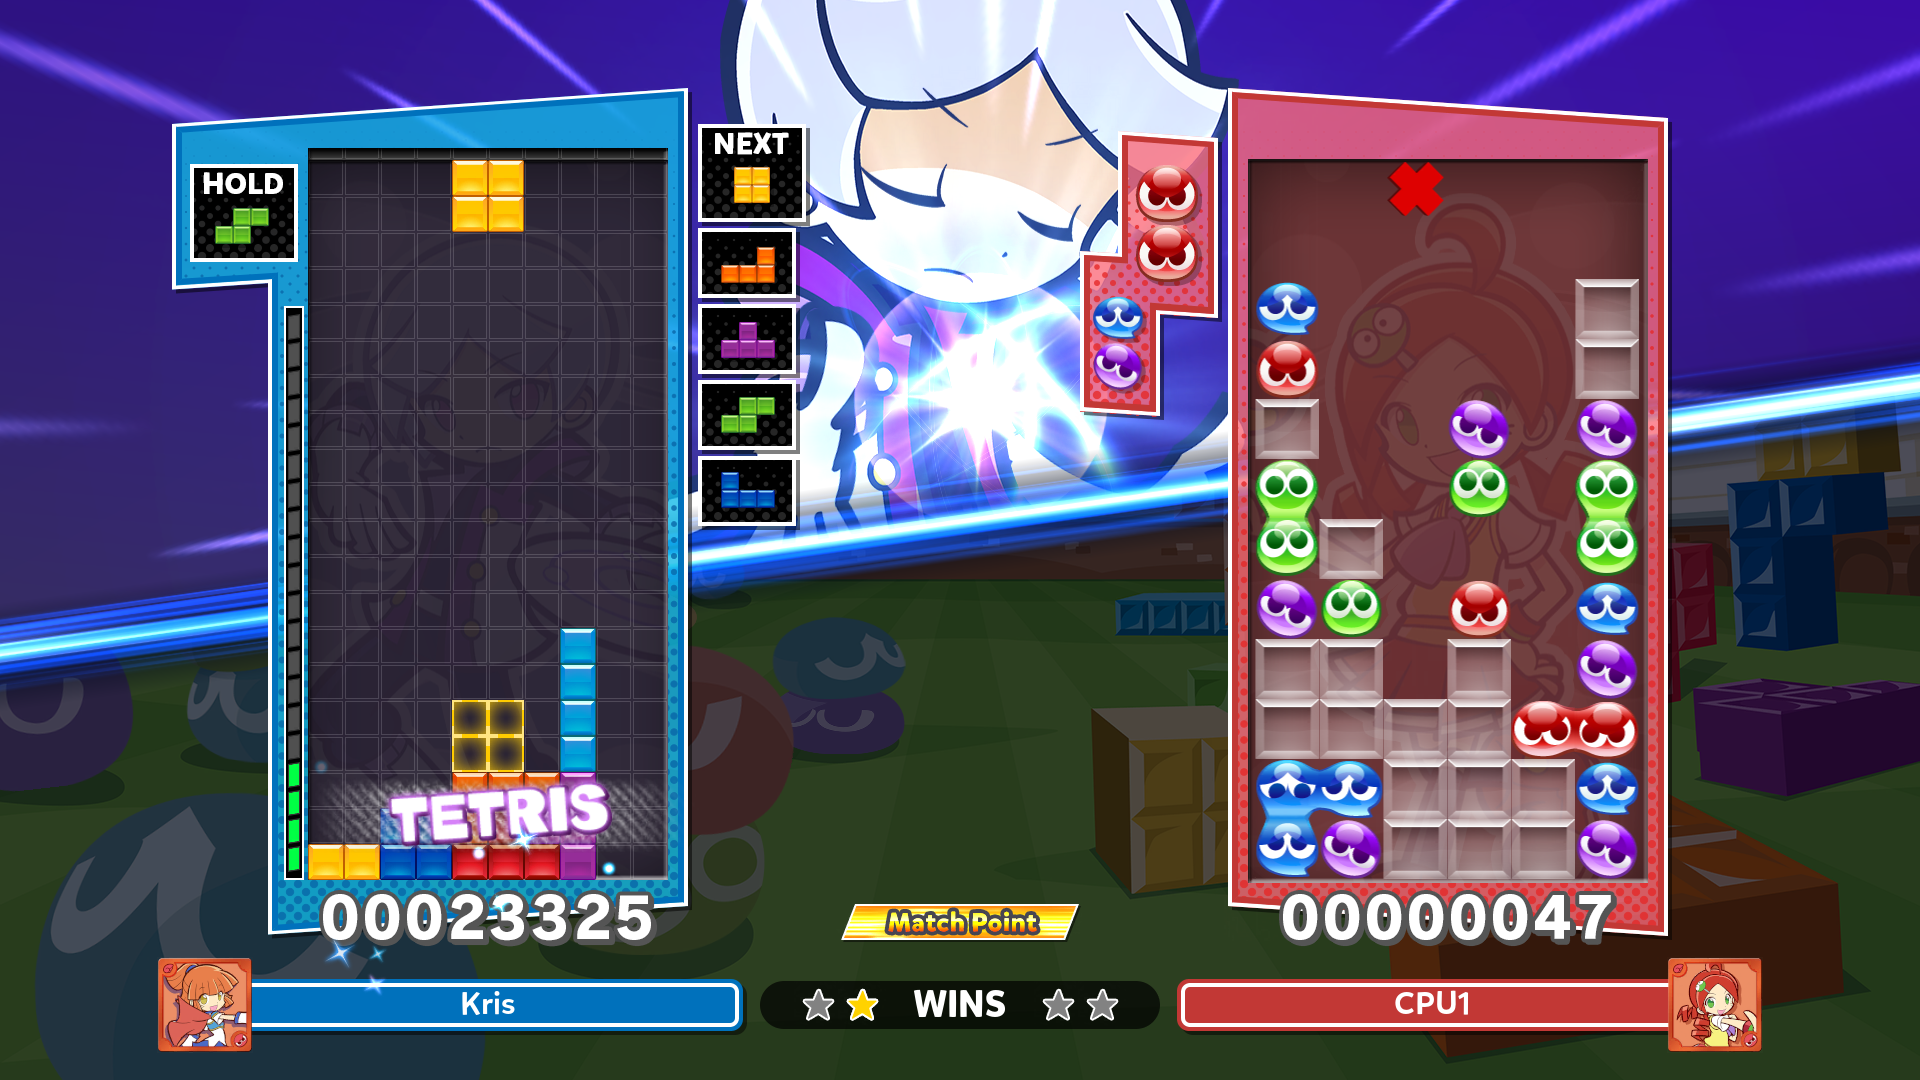
\includegraphics[width=1\textwidth]{ppt2.png}
\caption{\label{fig:ppt2}A screenshot of a versus battle, I'm playing Tetris and the CPU is playing Puyo Puyo.}
\end{figure}
Link: \href{https://store.steampowered.com/app/1259790/Puyo_Puyo_Tetris_2/}{https://store.steampowered.com/app/1259790/Puyo\_Puyo\_Tetris\_2/}

Puyo Puyo Tetris 2 is the latest Puyo Puyo game released by Sega and combines Puyo Puyo gameplay with Tetris, allowing players of both games to seamlessly play against one another. It has a full story and online mode.
\vspace{1cm}

Advantages:

\begin{itemize}
    \renewcommand\labelitemi{--}
    \item Cutesy art style is appealing to many, but can be swapped out with unlockable designs
    \item Being an official release, it is very stable with a consistent online multiplayer
    \item CPU opponents
    \item Fully voice-acted story with unique and creative characters
    \item Active modding community
\end{itemize}

Disadvantages: 

\begin{itemize}
    \renewcommand\labelitemi{--}
    \item Ranked multiplayer is fundamentally flawed as leaving matches is not punished
    \item CPU opponents fail to provide a challenge
    \item The game is very expensive, whereas all other options listed above are free
    \item Tsu ruleset, unable to be changed
\end{itemize}

\section{End User Input}

Being a popular game, many people enjoy the Puyo Puyo franchise, but the best people to survey for this project were the people who were most familiar with DRMBM specifically - speedrunners. A lot of the research in this document was greatly helped by the members of the "Puyo Speedrun" Discord server, and the contributers to the DRMBM-specific channel they have there.
In order to efficiently collect statistical end user input, a form was created using Microsoft Forms, a PDF version of which can be found here: \href{https://github.com/Kris-0605/nea/blob/master/documentation/Survey.pdf}{https://github.com/Kris-0605/nea/blob/master/documentation/Survey.pdf}

Question 1: Have you played Dr Robotnik's Mean Bean Machine before?
\begin{itemize}
    \renewcommand\labelitemi{--}
    \item Yes
    \item No
    \item Other Puyo Puyo game
\end{itemize}
Only one answer was permitted.

\begin{figure}[ht]
    \centering
    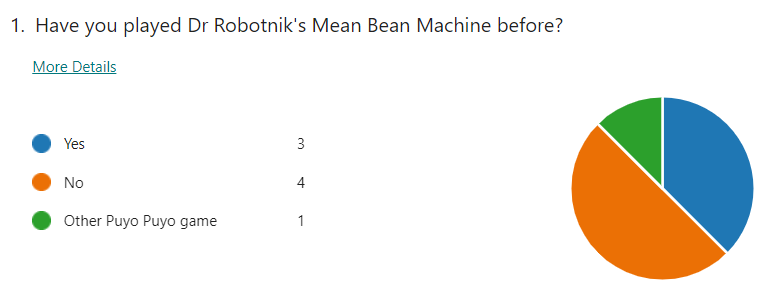
\includegraphics[width=0.8\textwidth]{survey1.png}
    \caption{\label{fig:survey1}Results to the first survey question.}
\end{figure}

The only notable thing about this question is that anyone who answered "No" was taken to the end of the form and was unable to answer any other questions. Thus, only 4 people continued to fill out the rest of the form.
\\\\
Question 2: Which modes in DRMBM are you experienced with and enjoy using?
\begin{itemize}
    \renewcommand\labelitemi{--}
    \item Scenario mode
    \item 1P VS. 2P mode
    \item Exercise mode
    \item Other
\end{itemize}
Any number of answers were pemitted.

\begin{figure}[ht]
    \centering
    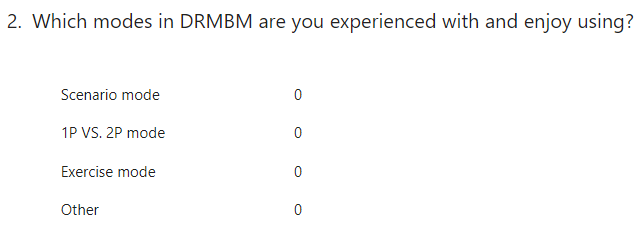
\includegraphics[width=0.8\textwidth]{survey2.png}
    \caption{\label{fig:survey2}Results to the second survey question.}
\end{figure}

No-one answered this question, thus nothing meaningful is gained from it.
\\\\
Structure
"This project is intended to both remake the original game in it's purest form, apply enhancements to it, thus the game will be split into two modes, that will from now on be referred to as "Classic mode" and "Enhanced mode". Classic mode is intended to be an exact recreation of the original game, and Enhanced mode should contain any additions and improvements."
\\\\
A message explaining some of the games structure that is important to understand when considering survey questions, which will be discussed further in the documented design section.
\\\\
Question 3: Consider scenario mode's password feature. Enhanced mode will allow the player to use save files that store additional data such as score, times and replays. What do you believe is the best way for the password menu to be implemented?
\begin{itemize}
    \renewcommand\labelitemi{--}
    \item Classic mode will use the same passwords from the original game in their original form, taking you to a level but not restoring data such as score
    \item Classic mode will generate new unique password that stores a hidden save file, so that the user is still required to use a password, but this password restores data such as score when used
    \item The password menu should be entirely replaced by save files in both modes
    \item Other
\end{itemize}
Only one answer was permitted.

\begin{figure}[ht]
    \centering
    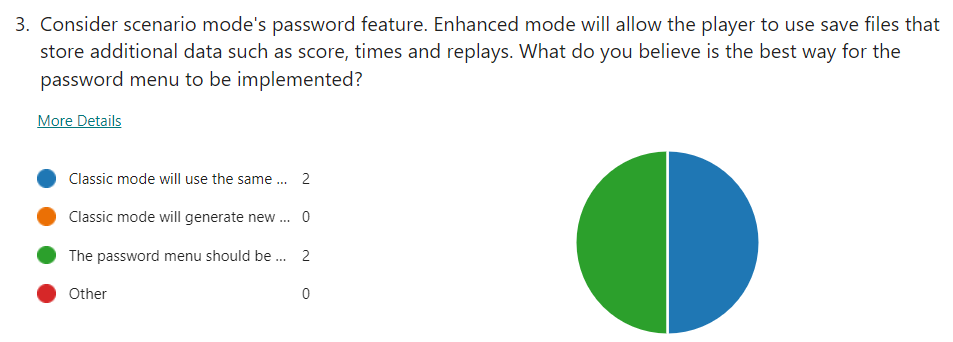
\includegraphics[width=0.8\textwidth]{survey3.png}
    \caption{\label{fig:survey3}Results to the third survey question.}
\end{figure}

The results to this question were an exact 50/50 split, thus I shall stick to my original plan of having Classic mode use passwords in their original form without any additional data, and using save files for enhanced mode.
\\\\
Question 4: What is your opinion on scenario mode's difficulty?
\begin{itemize}
    \renewcommand\labelitemi{--}
    \item Harder modes should be added to challenge more difficult players
    \item Easier modes should be added to help new players
    \item The difficulty options should remain the same in scenario mode, more customisable opponents should be available in a separate "training mode" in enhanced mode
    \item I don't believe any changes should be made
    \item Other
\end{itemize}
Any number of answers were pemitted.

\begin{figure}[ht]
    \centering
    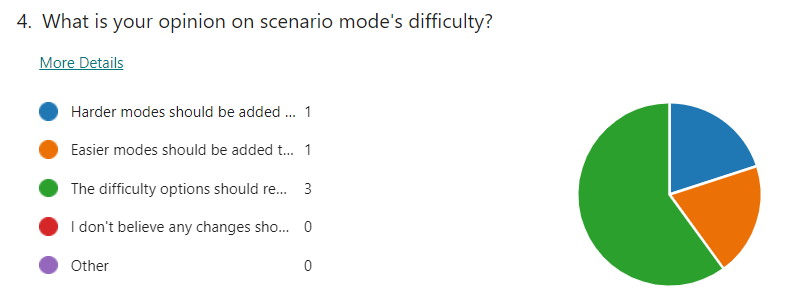
\includegraphics[width=0.8\textwidth]{survey4.png}
    \caption{\label{fig:survey4}Results to the fourth survey question.}
\end{figure}

The majority vote represented the solution that I believe would fit best and already planned on implementing: in both classic and enhanced mode, difficulty shall remain the same as in the original. However, in enhanced mode, you can play against customisable opponents, such as the same algorithms from scenario mode with different speeds, as well as new AI altogether.
\\\\
Question 5: The original game uses the OPP ruleset for scenario mode, the main difference being that garbage cannot be cancelled. What do you believe is the best configuration of rulesets?
\begin{itemize}
    \renewcommand\labelitemi{--}
    \item Classic mode scenario mode should use the OPP ruleset to recreate the original game and Enhanced mode should allow the user to choose before starting a save file
    \item Force OPP for scenario mode in both modes and allow players to choose Tsu when creating custom games
    \item Other
\end{itemize}
Only one answer was permitted.

\begin{figure}[ht]
    \centering
    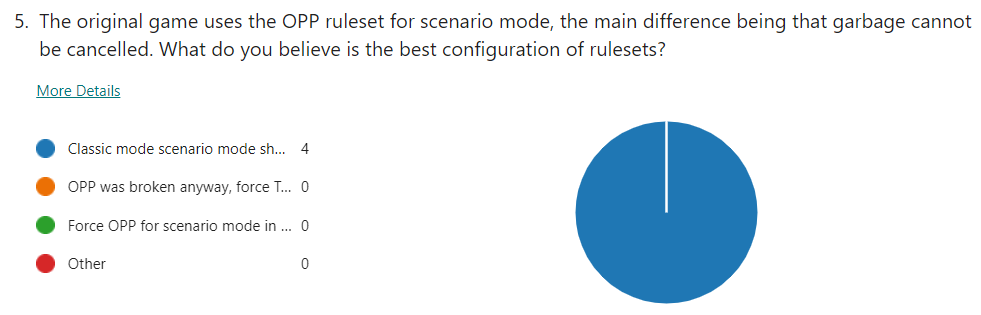
\includegraphics[width=0.8\textwidth]{survey5.png}
    \caption{\label{fig:survey5}Results to the fifth survey question.}
\end{figure}

The only unanimous result in the entire survey, as well as the solution I was planning on implementing. I will talk more about rulesets in the documented design section.
\\\\
Question 6: Do you have any other additions or comments regarding scenario mode?
This question permitted a text answer.

\begin{figure}[ht]
    \centering
    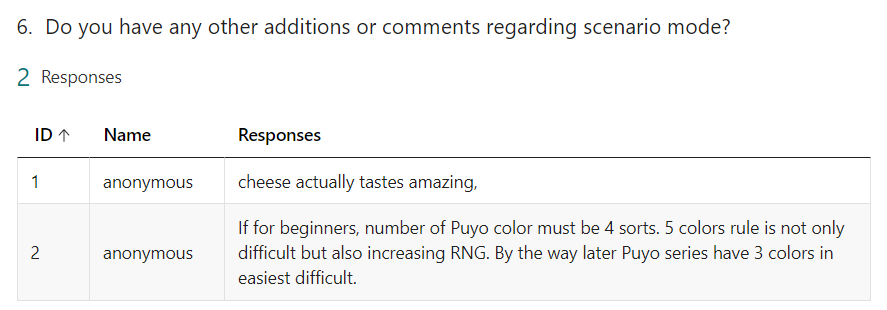
\includegraphics[width=0.8\textwidth]{survey6.png}
    \caption{\label{fig:survey6}Results to the sixth survey question.}
\end{figure}

Response ID 2 makes a very valid point. In newer versions of puyo puyo, difficulty settings change the number of colours that appear in play between 3, 4 and 5, whereas being an older game DRMBM uses 5 puyo colours in all difficulty modes. I will be sure to include the suggestion in enhanced mode.
\\\\
Question 7: While ambitious, the plan is to eventually include online multiplayer in the game for enhanced mode. Which of the following modes would you be interested in using? 
\begin{itemize}
    \renewcommand\labelitemi{--}
    \item Customisable private rooms that you can invite other players to
    \item Customisable public rooms, given in a listing that anyone can join
    \item Ranked multiplayer, with a rating system
    \item A super lobby (i.e. 20+ players)
    \item Other
\end{itemize}
Any number of answers were pemitted.

\begin{figure}[ht]
    \centering
    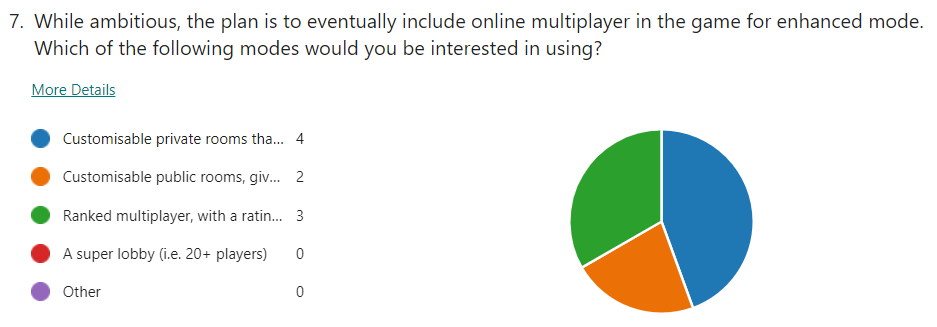
\includegraphics[width=0.8\textwidth]{survey7.png}
    \caption{\label{fig:survey7}Results to the seventh survey question.}
\end{figure}

All of the above are planned to be implemented, but the distribution of votes gives me a timeline with which to work on each feature.
\\\\
Question 8: When considering the Has Bean and Big Bean bonuses in exercise mode, which of the following statements do you agree with?
\begin{itemize}
    \renewcommand\labelitemi{--}
    \item Has Bean and Big Bean should be toggleable when playing exercise mode in enhanced mode
    \item Exercise mode attempts using Has Bean and Big Bean should use a separate leaderboard
    \item Has Bean and Big Bean should always be forced in exercise mode since they are part of the game mode, and should be toggleable when playing custom games
    \item Other
\end{itemize}
Any number of answers were pemitted.

\begin{figure}[ht]
    \centering
    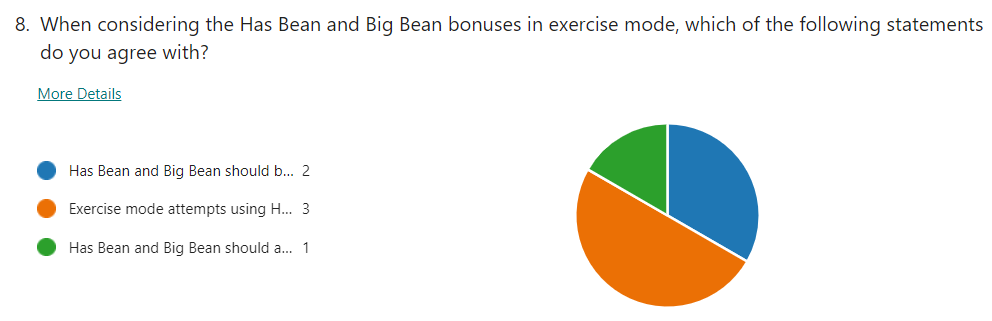
\includegraphics[width=0.8\textwidth]{survey8.png}
    \caption{\label{fig:survey8}Results to the eighth survey question.}
\end{figure}

The majority of people would like leaderboards to be split between runs that use Has Bean/Big Bean and runs that do not. This is surprising to me, but not particularly difficult to implement thus shall be included. This overrides the one person's comment about always forcing them.
\\\\
Question 9: In DRMBM, the score counter is capped at 99,999,999, and the puyo counter is capped at 9,999. In the original game, these counters froze on the event of a max out. How do you think a max out should be handled?
\begin{itemize}
    \renewcommand\labelitemi{--}
    \item In Classic mode, the counter should freeze, in Enhanced mode the counter should physically expand to accommodate more digits
    \item The counter should always freeze
    \item The counter should always expand
    \item Other
\end{itemize}
Only one answer was permitted.

\begin{figure}[ht]
    \centering
    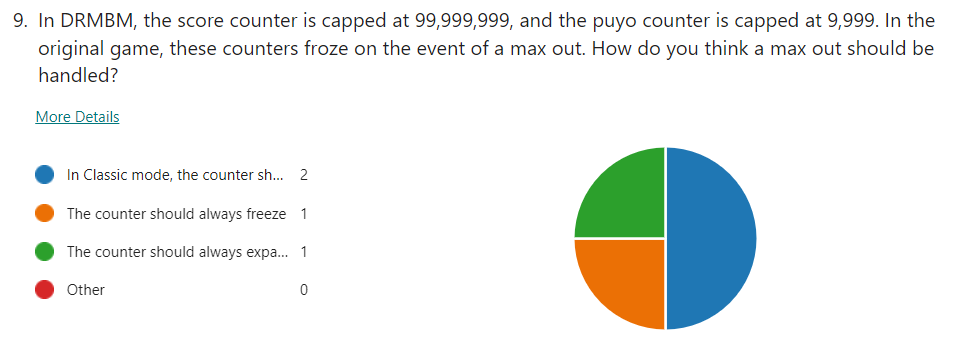
\includegraphics[width=0.8\textwidth]{survey9.png}
    \caption{\label{fig:survey9}Results to the ninth survey question.}
\end{figure}

A majority of people would like to implement the solution that I personally had in mind: freezing the counters in classic mode and allowing them to physically expand in enhanced mode, so this is what I shall implement. I understood that allowing the counters to freeze in classic mode would be important to keep because a popular speedrun of the game is trying to max out the score counter in the least possible time, and removing this bug would take away from one of the ways people enjoy the game.
\\\\
Question 10: As part of the project's requirements, I am going to include an online leaderboard. What stats do you think should be available as a leaderboard?
This question permitted a text answer.

\begin{figure}[ht]
    \centering
    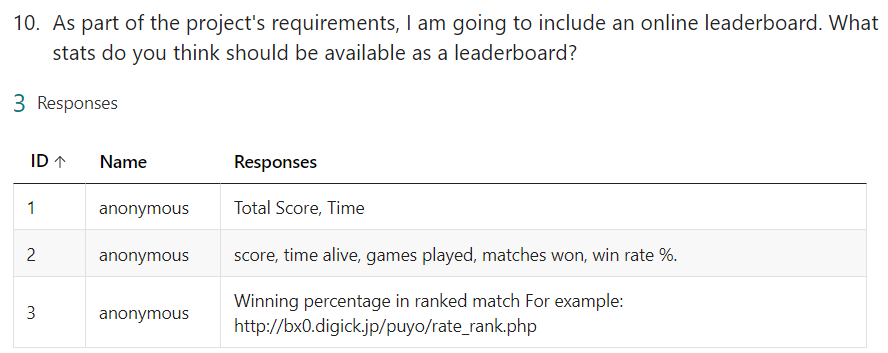
\includegraphics[width=0.8\textwidth]{survey10.png}
    \caption{\label{fig:survey10}Results to the tenth survey question.}
\end{figure}

These are all fairly generic examples, but I do appreciate the link provided to a Japanese ranked BPuyo leaderboard to use as an example.

\begin{figure}[ht]
    \centering
    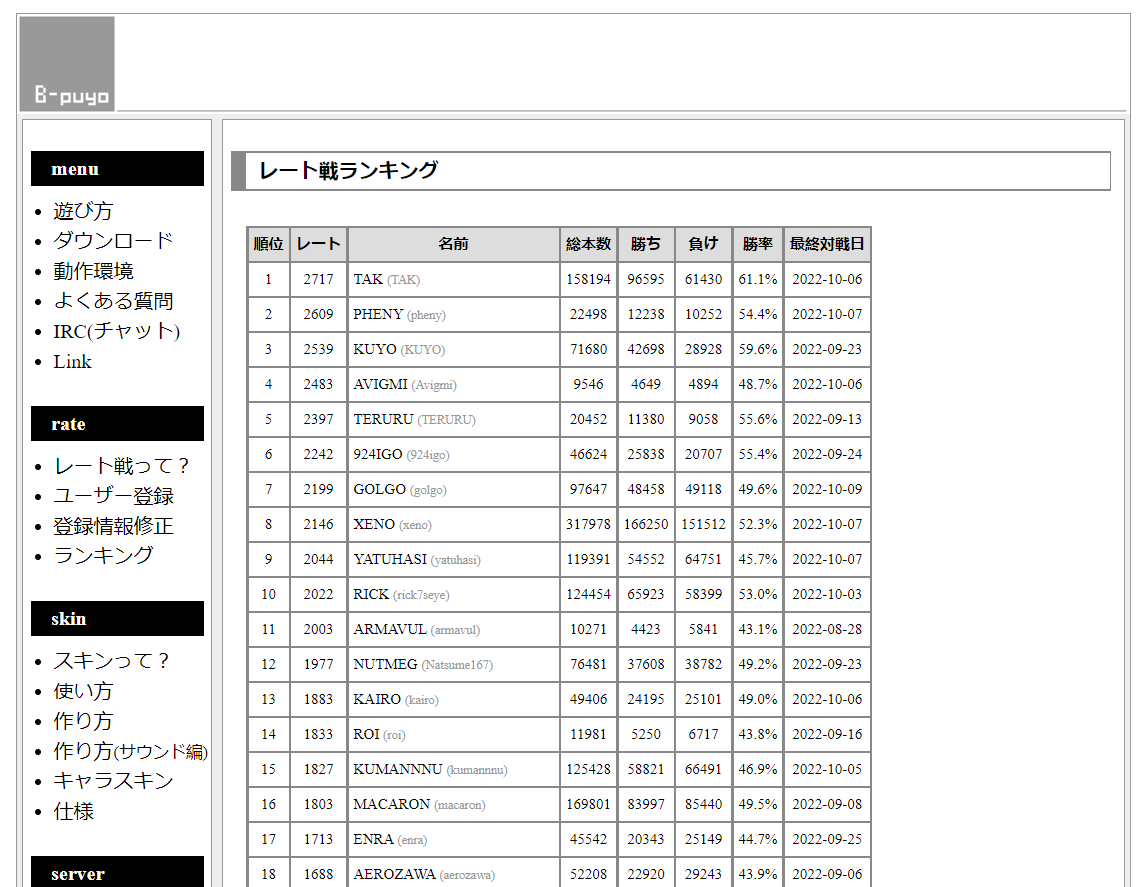
\includegraphics[width=0.8\textwidth]{bpuyo_leaderboard.png}
    \caption{\label{fig:bpuyo_leaderboard}The ranked leaderboard from the Bpuyo website.}
\end{figure}

Question 11: Enhanced mode will allow the game to support a 16:9 aspect ratio. What do you believe should be used to fill the space?
This question permitted a text answer.

\begin{figure}[ht]
    \centering
    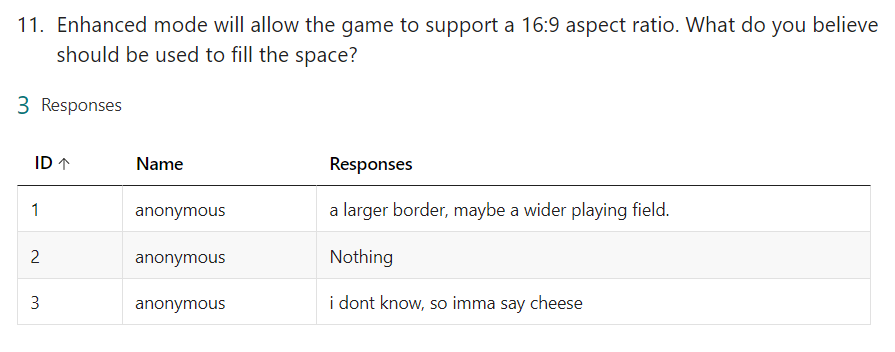
\includegraphics[width=0.8\textwidth]{survey11.png}
    \caption{\label{fig:survey11}Results to the eleventh survey question.}
\end{figure}

The solution to this problem remains to be determined, so I will probably fill it with empty space for now and see if I figure out something convenient later.
\\\\
Question 12: Below are other features that I plan to implement into Enhanced mode. Rate their importance.
The options contained within rows were:
\begin{itemize}
    \renewcommand\labelitemi{--}
    \item Custom texture support
    \item Custom handling settings
    \item Custom resolutions (any aspect ratio)
    \item Allow for custom AI and bots
    \item Simple modding API, mod installation built-in to the game
\end{itemize}
The options contained within columns were:
\begin{itemize}
    \renewcommand\labelitemi{--}
    \item I actively dislike this
    \item Would be nice to have, but not needed
    \item Should be included in final release
    \item Critical, prioritise this!
\end{itemize}

\begin{figure}[ht]
    \centering
    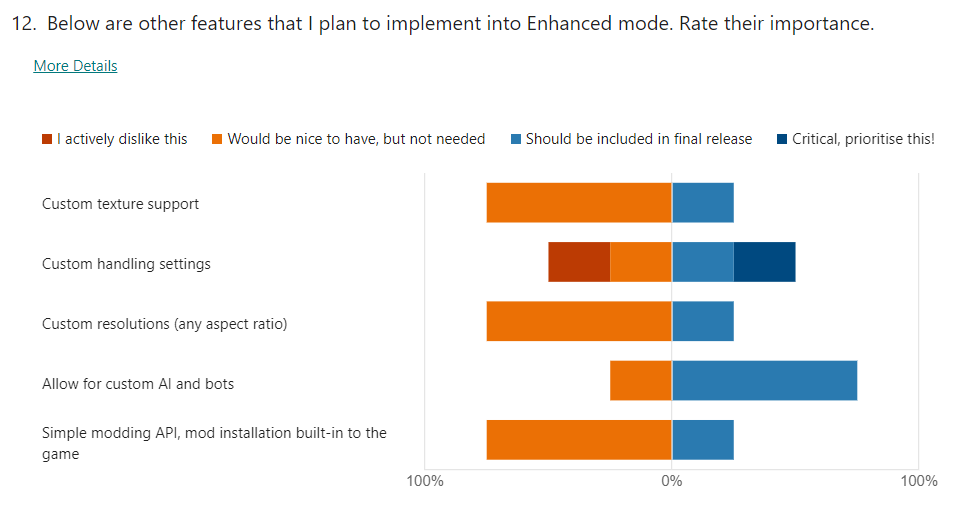
\includegraphics[width=0.8\textwidth]{survey12.png}
    \caption{\label{fig:survey12}Results to the twelth survey question.}
\end{figure}

All of the items listed are planned to be included, it is simply a matter of prioritising what the end user considers important.
For custom textures, 3 people said it would be nice to have and 1 said it should be in the final release. The inclusion of custom texture support itself is fairly trivial to implement due to the nature of having to import textures using the engine anyway, the time-consuming part would be writing documentation that explains how people can create their own texture packs that would be compatible with the game. I now know that this should not be prioritised.

Custom handling settings was the most devisive option, with each of the 4 applicants choosing separate options. I don't understand the rational behind actively disliking custom handling settings as the default will be the same as they are in the actual game, however it may be worth considering forcing certain handling settings in ranked matches or games that will be displayed on leaderboards; perhaps different leaderboards with enforced handling and custom handling? This will have to be considered.

Custom resolutions received the same reception as custom textures - it would be nice to have but isn't overly important. Different aspect ratios are actually especially challenging and non-trivial to implement. My original design for the engine involved scene data containing a background image variable, however this static image doesn't account for different resolutions and aspect ratios. Thus in order to account for future support for multiple aspect ratios, the engine must be coded to accept the background as a function that draws the background. Then when coding scenes, the specific scene can decide the solution that is most appropriate for drawing the background, whether that be a solid colour, stretching an image to fit a resolution, having multiple images to support multiple aspect ratios or some kind of tiling solution.

Custom AI and bots received a positive reception. I shall have to create an object that allows for the implementation of AI to create the CPUs in scenario mode, thus it shall be trivial to allow modders to run their own function within this class (with some kind of primitive virus protection by not allowing external modules to be accessed).

The described "modding API" will simply be an expanded version of what is described above - allowing users to modify their game by importing new objects written by other users that are compatible with the engine, at the user's own risk.

The survey was supposed to include a poll about replays, but unfortunately I forgot to include it. I can only assume it would be a desired feature.

\section{Input, Data Processing, Output}

The program is started with main.py. This script shall verify the integrity of local game assets using SHA hashing and querying a simple API on a web server, retrieving assets as necessary. Then, the script shall import Kris's Engine, an engine that shall be written and packaged by me with the game. 

Kris's Engine is built upon the idea of two fundamental class templates Scene and Entity, which shall be further described within the Documented Design section of this report. The engine shall first initalise itself, loading textures and initialising modules such as aiohttp and pygame. The engine shall then import the scene that is predefined by main.py, which will probably be title.py to load the title screen. From then, the engine shall use two threads: one for rendering and one for updating entities. Each entity must have the methods render and update, where the engine on seperate threads will call update 600 times per second and render a variable amount of time, that is able to be changed by the user, that will default to 60. The update method for an entity is responsible for data processing and the render method is responsible for any visual output that may be needed.

\begin{figure}[ht]
\centering
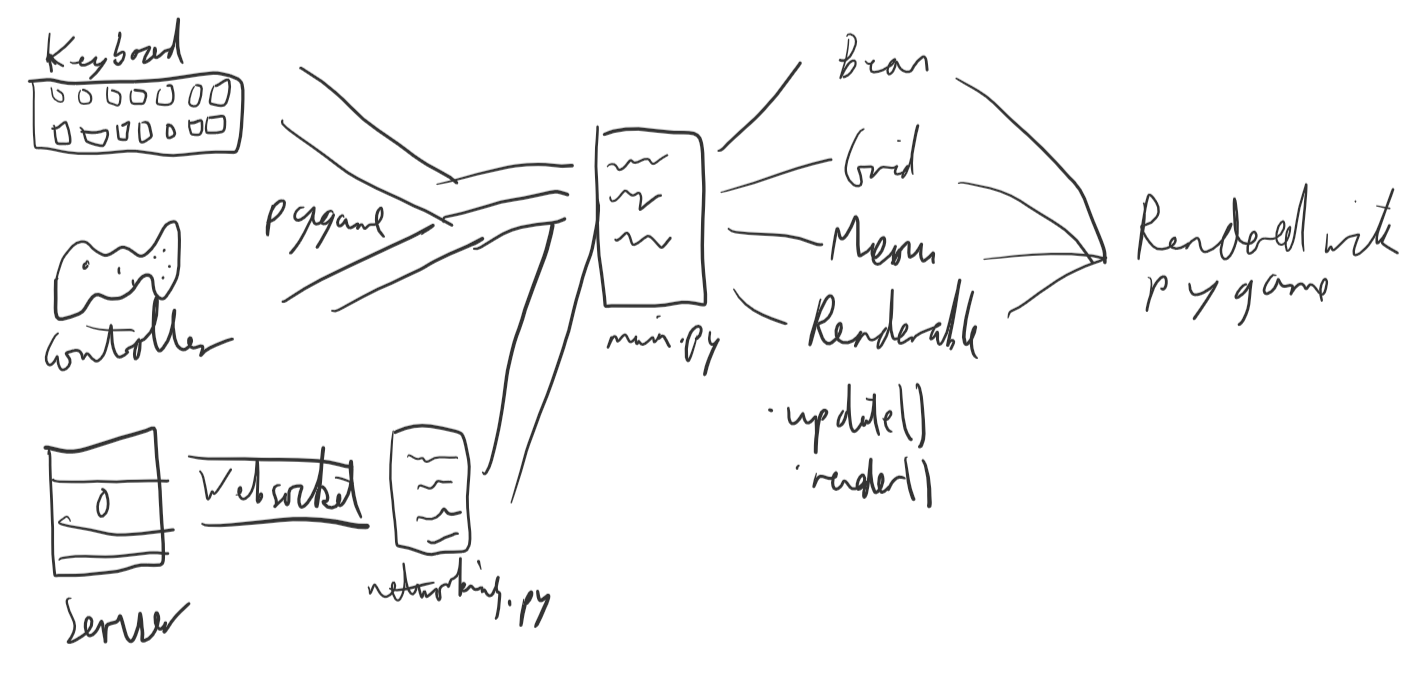
\includegraphics[width=1\textwidth]{idpo.png}
\caption{\label{fig:idpo}An Input, Data Processing, Output diagram.}
\end{figure}

\subsection{Goals}

\subsubsection{Main objectives}

\begin{itemize}
    \renewcommand\labelitemi{--}
    \item The project shall contain an engine module, which consists of an Engine class. This Engine class should:
    \begin{itemize}
        \renewcommand\labelitemi{--}
        \item Define the Scene and Entity classes, to be used as templates. These objects will be described further in depth in this document's Documented Design section.
        \begin{itemize}
            \item The Scene class should allow an object that inherits from it to:
            \begin{itemize}
                \item define what assets (images, sound files, etc) need to be present for a given scene.
                \item define some functions required for rendering a scene such as a function for rendering the background of a scene that works for different resolutions
                \item define what entities should be loaded in with a scene, their order and initialisation parameters
            \end{itemize} 
            \item Any object that inherits from the Entity class should:
            \begin{itemize}
                \item Define an update method which handles the data processing for a given entity.
                \item Define a render method which handles the output for a given entity, be that pygame rendering functions, console print statements, logging to a file, etc.
            \end{itemize}
        \end{itemize}
        \item Initialise pygame and take ownership of all pygame objects, such as the screen object being located at Engine.screen
        \item Initialise two threads:
            \begin{itemize}
                \item A thread shall be responsible for handling the update method of every entity that is owned by the engine. The aim is to run this 600 times per second.
                \item A thread shall be responsible for handling the render method of every entity that is owned by the engine. The aim is to run this at least 60 times per second, however due to the constant rate of the update function, this could be ran at any speed without affecting any game logic. For this reason, counter-intuitively it is critical that things that must be done at a constant rate, such as animations, rely on the update function instead of the render function, and the render function should be used only for drawing.
            \end{itemize}
        \item Contain a method for loading scenes that entities can invoke
        \item Contain methods that allow entites to easily make requests without causing the program to freeze
        \item Contain methods for handling backend tasks such as changing resolution, setting the window to fullscreen, etc.
        \item Contain methods for easily playing sounds on different channels. The engine is responsible for ensuring that a sound can always be played and that the number of pygame mixer channels is never exceeded.
        \item The engine could contain generic methods that prevent repeating complex code, for example a method that creates a spray of particles. This is something that would be time consuming to implement into every entity that requires it and would be incredibly resource intensive if an entity was used for each particle, thus it makes sense to have it as a function that can be used by any program that uses the engine, with a replaceable texture.
    \end{itemize}
    \item The game shall be split into two modes, Classic mode and Enhanced mode.
    \begin{itemize}
        \item Classic mode shall attempt to be a faithful recreation of the original game. This includes:
        \begin{itemize}
            \item A recreation of all 13 stages in "scenario mode", the game's equivalent of a story mode. Various algorithms are used for your computer opponents and an attempt shall be made to recreate these algorithms as faithfully as possible, though lack of documentations means that some compromises will have to be made.
            \item "excercise mode" should function as in the original, with three speed difficulties, counters for score and difficulty, and the spawning of the Has Bean and Big Bean power-ups. Two simulatenous, separate games should be supported, allowing to players to play locally on the same device independantly.
            \item "1P VS. 2P mode" should have the original 5 difficulty modes and two players should be able to use separate input devices to play two linked games in a competitive match locally.
            \item An "options" menu. This will only contain the the settings found in the original settings menu, other settings shall be found in the menu found when the game starts up for selecting between Classic and Enhanced mode. 
        \end{itemize}
        \item Classic mode shall be developed first, and Enhanced mode will be built upon Classic mode. The aim is to include the following changes:
        \begin{itemize}
            \item A customisable resolution. Certain scenes such as the animated segments before levels in scenario mode will need to be locked to certain aspect ratios such as 4:3 or 16:9 in order to look correct, whereas other scenes can function at any aspect ratio. Due to pygame not allowing windows to be resizeable, there will have to be a setting to allow the user to change the resolution, and locked aspect ratios shall be achieved by black bars, which will be rendered by the background method of a given scene object.
            \item The ability to store and play replays of games from any mode.
            \item Save files for scenario mode.
            \item The ability to customise handling, such as the amount of time before a bean starts to repeat movement when the left or right key is pressed down (this is a value known as "DAS")
            \item An online leaderboard in excercise mode. This will function using a simple script running on an external, central web server. The leaderboard should use an SQL database to store user information, locations of replay files and information such as scores and times. The leaderboard factor will be implemented using a merge sort algorithm to sort scores into the correct order. The user should be able to easily play the replays of users on the leaderboard. As requested from end user input, there shall be separate leaderboards for attempts that make use of the now toggleable Has Bean and Big Bean powerups, as well as separate leaderboards for users who choose to use custom handling.
            \item General bug fixes should be implemented such as, as requested during end user input, the score counter in excercise mode should expand to allow for scores greater than 100 million.
            \item Implementation of the Tsu ruleset. The Tsu ruleset includes rules such as the cancellation of pending garbage beans and bonuses for things like perfect clears. When creating a save file the user should be asked which ruleset they want to use.
            \item Allow the user accessibility to the games underlying classes so they can easily modify the game with things such as custom textures and importing their own AI opponents.
        \end{itemize}
    \end{itemize}
\end{itemize}

\subsection{Extension objectives}

If the project goes well, the aim is to include:
\begin{itemize}
    \renewcommand\labelitemi{--}
    \item Real-time online multiplayer using web sockets.
    \item Implementation of my own custom AI.
\end{itemize} 

\chapter{Documented Design}

\section{Language and rendering module}

The project shall be written in Python 3 because it is the language I have the most experience with. The third-party Pygame module shall be used for rendering graphics to the screen because of it's well-written documentation and ease-of-use.

\section{Engine classes}

When creating a game, it is important to create a generalised, versatile and reusable structure. Additionally, performance and consistent timing of backend tasks are important to this project. Thus, before approaching the game I first created a module that would be helpful in the game's development by containing code and classes that would be consistently reused. This module, which I will refer to as the engine module, contains three main classes: Engine, Entity and Scene. Entities are things individual things that need to be drawn on screen or processed, a Scene object defines reusable functions and information about how entities should be defined and an Engine object has a relationship of aggregation with Scenes and Entities, is capable of loading and destroyed them, and handles backend and threading tasks.

\subsection{Entity}

An Entity is a base class that is designed to be inherited from to quickly implement new types of objects on screen or that need to be processed. It has the following attributes and methods:

\subsubsection{persist}

The Entity class defines persist to be False by default, but it could be changed to True by someone creating an entity. If persist is set to False, then when the engine loads a new scene, the entity will be destroyed. If persist is true, it will remain throughout different scenes until explicitely destroyed.

\subsubsection{\_\_init\_\_}

This method has the parameters engine, scene and id. It expects the inputs to these parameters to be the engine object, the scene object that is creating the entity, and a unique integer ID. This function should be overwritten so that a developer may initialise their own entity, and the developer is expected to maintain these three positional arguments in this order, in addition to adding their own arguments and keyword arguments. A developer can easily execute this \_\_init\_\_ function in addition to their own by running "super().\_\_init\_\_(engine, scene, id)"

\subsubsection{init}

This method should largely be ignored and is used initialise the attributes of the default Entity in the case that this class was to be initialised directly instead of being inherited from. Loading Entity directly creates a spinning square.

\subsubsection{update}

A developer is expected to override this function. It is executed at a set rate by the update thread, explained more in the Engine class section. It should be used for backend tasks, and tasks that need to happen at a constant rate such as animations.

\subsubsection{render}

A developer is expected to override this function. It is executed every time a frame is rendered and therefore should not be expected to run at a constant rate. This function should not complete any backend tasks and should instead draw on screen with pygame functions a representation of what is happening in the backend.

\subsection{Scene}

A Scene is a base class that is designed to be inherited from to easily implement the loading of many entities. An example of this would be transitioning from a menu to gameplay by loading the gameplay scene, destroying the entities from the menu scene It has the following attributes and methods:

\subsubsection{load\_with\_pbar}

This attribute should be an iterable such as a list or tuple. If filled with filenames, then before the loading of this scene, a built-in progress bar scene will be used to load the files listed into the engine's asset cache.

\subsubsection{update\_rate}

This attribute should be a positive non-zero integer, and represents the number of updates per second the engine will attempt to execute for the duration of the scene. Since tasks are designed to expect a constant rate from this number, halving this number would create the effect of running a scene's backend at half speed, and drastically reducing it would make the scene appear to be running in slow motion.

\subsubsection{render\_rate}

This attribute should be a positive integer, and represents the number of frames per second the engine will attempt to render for the duration of the scene. Reducing this number would make the scene's backend still run at the same speed, but the output would appear choppy. Setting this number to 0 will cause the engine to try and render as many frames as possible without waiting.

\subsubsection{background}

background is both an attribute and a method. It is expected that background be a function object, but by default this is implemented as a lambda function assigned to a variable. background will be called every frame before entities are rendered and by default will fill the screen with black, clearing it.

\subsubsection{music}

Another combination between an attribute and a method, music is a function that should return a pygame Sound object. This sound will then loop until another scene is loaded.

\subsubsection{kap}

This attribute should be an iterable, such as a list or tuple, of strings. When loading the scene, the engine will ensure that all the KAP files listed are loaded to ensure that textures are accessible. KAP files will be explained later in this section.

\subsubsection{\_\_init\_\_}

This method is expected to be overrided. Its only positional argument is engine, expecting the engine object that is loading the scene, which is then assigned to self.engine. A developer can either implement this by running "super().\_\_init\_\_(engine)", or just running "self.engine = engine".

\subsection{Engine}

The Engine contains many methods and serves many purposes. The main purpose of the engine is to manage a multi-threaded structure. Updates and rendering are handled independantly on different threads at different rates. This is done to allow them to run at different rates, as well as to allow for an uncapped frame rate and improved performance in such a performance-critical genre such as stacker games.

\subsubsection{\_\_init\_\_}

This method has many keyword arguments.
\begin{itemize}
    \item scene represents the scene that the engine should load. If none is given, the default Scene class is initialised.
    \item width and height represent the pixel size of the window
    \item engine\_path and log\_path are used to specify the location of files relative to the programs current point of execution
    \item texture\_quality controls the resolution at which image textures are loaded, using this feature of KAP files
    \item log\_max\_size specifies a maximum size for the log file before it begins to be trimmed from the top. This defaults to 10MB.
\end{itemize}

All of these are stored in private variables that can be access but not written to, with the exception of texture\_quality, which has a setter than flushes the engine's asset cache when the texture\_quality is changed in order to load the textures of a new quality.

This function initialises id, a getter that increments the id attribute for creating unique entity IDs.

The logging thread is then initialised.

The now depreciated config file is then loaded.

Some timers are set and attributes are defined, then pygame is initialised.

Default assets, to be used if an asset it missing, are loaded.

More attributes are defined and the pygame window is created.

The update and render threads will be started, and the specified scene will be loaded.

Then, the engine will collect pygame events, using event\_gotten to synchronise with frames on the render thread, until the program exits when pygame will be quit and the main thread will terminate.

\subsubsection{init\_log}

Printing in python is slow. The logging thread periodically flushes log messages to the console, flushing multiple messages at a constant interval to save on processing time. These messages are in a constant format detailing the time since execution of the program began, and colour coding messages with ANSI escape codes, the colour being dependant on the thread the message was made with. Additionally a separate log is kept without ANSI escape codes to be stored in a text file.

This method creates the necessary variables for this system to function, and starts the thread that dumps the log to the console. It has no parameters.

\subsubsection{loop\_log}

The method that is passed to the thread for execution until the program is terminated. This method outputs the log to the console and then waits for a period of time specified in init\_log. Sleeping in a thread only pauses that thread, so this allows other execution to continue. It has no parameters.

\subsubsection{exit\_log}

This method uses Python's "atexit" module to write the log to a text file when the program is terminated. It has no parameters.

\subsubsection{append\_log}

This method takes a message (a string) as a parameter and formats a log message by getting information about the current thread and current time.

\subsubsection{load\_config}

This method used to be used to load the information that is now specified by keyword variables. It is no longer used, but can be used by a developer if they wish to load additional settings. It looks for a config.json file and if it exists, assigns the contents of the file to a config dictionary attribute. It has no parameters.

\subsubsection{save\_config}

This method saves the content of the config parameter to a JSON file. It has no parameters.

\subsubsection{get\_events}

This method is used to fetch pygame events and put them into a list, the events attribute. It also checks for a pygame.QUIT event, which happens when the close button is pressed on the window. This sets the running attribute to False. All threads should use "while self.running" for any infinite loops, meaning that they will finish executing that iteration and then terminate when self.running is set to False. This function has no parameters.

\subsubsection{get\_asset}

This method is accepts a filename as a required parameter. It will either load the given file into a cache (at the assets attribute, or the font\_assets attribute), or load it from the cache if it is already there. It will return a pygame object version of the specified file. So, if audio is set to True, then a pygame.mixer.Sound object is returned. If font is set to an integer then a version of that font rendered at the given font size is returned as a pygame.font.Font object. Otherwise, a pygame surface object is returned. This function can also scale image textures using the \_\_scale method and store the scaled copies, to prevent scaling being done frequently. Additionally, if a given filename is not found in an loaded KAP files, this function will return an alternative of the same filetype from "default.kap" in the engine folder.

\subsubsection{\_\_scale}

Accepts two positional arguments, scale and path. scale can be one of three types: a string "raw", a tuple containing a width and height for the image to be scaled to, or a float. If a float is provided, then the image will maintain it's original asepct ratio, and be scaled such that the height is equal to the float specified multiplied by the window height of the engine.

\subsubsection{load\_entity}

This method accepts an entity and a scene as positional arguments, as well as allowing for additonal arguments and keyword arguments to be passed into the entity upon it's initialisation. scene should be an initialised scene object while entity should be a class that hasn't been initialised yet. First this method will verify that the class given has inherited from the Entity class, then it will generate a unique ID, initialise the entity and store it, creating a relationship of aggregation between the Grid and the entity. It will then return the entity object.

\subsubsection{destroy\_entity}

Takes a single positional argument, being an initialised entity object. First the method verifies that the object passed in inherited from the Entity class, then it removes it from the entity list and dictionary of entity IDs. This is the only way to destroy an entity with persist set to True. This method will fail if the passed in entity is no longer owned by the engine.

\subsubsection{load\_scene}

This takes a positional argument, being a not-yet-initialised class that inherited from Scene. pbar is a keyword argument that needs to be set to False by a progress bar when trying to load a scene that has been loaded with a progress bar to prevent an infinite loop of calling the progress bar, otherwise it should be left alone. All other arguments and keyword arguments are passed into the scene upon initialisation.
First, this method sets the ready attribute to False, which pauses the update and render threads. Then, it verifies that the class being passed in inherited from the Scene class. Then, it will load all the KAP files given by the kap attribute of the scene. Then, it will destroy all non-persistant entities from the last scene. Then, if the pbar keyword is set to True and the scene has files in the load\_with\_pbar attribute, then the progress bar class is loaded for loading the files. Otherwise, other attributes from the scene are processed, the scene object is initialised, timers are reset and the update and render threads are unpaused.

\subsubsection{\_\_size}

A method used for calculating the amount to increment the progress bar by for a given file, by using its compressed size. It takes a single argument, being the file name.

\subsubsection{update\_loop}

This is a method that takes no arguments and is executed by the update thread. First, it assigns itself a colour, and then loops while the running attribute is True. Then, it does nothing if ready is set to False, to pause execution while a scene is being loaded. If ready is True, then the update\_counter attribute is incremented. For every entity in the ordered entity list, the update method is called. Then, the events attribute, a list of pygame events, is trimmed to remove the events that have already been process. Finally, the method calculates how long it needs to wait for to maintain a constant update rate, and outputs a lag message every two seconds if it detects that it is behind.

\subsubsection{render\_loop}

This is a method that takes no arguments and is executed by the render thread. First, it assigns itself a colour, and then loops while the running attribute is True. Then, it does nothing if ready is set to False, to pause execution while a scene is being loaded. If ready is True, then the render\_counter attribute is incremented. The background method for the currently loaded scene is called to clear the scene. Then, for every entity in the ordered entity list, the render method is called. Then, the thread waits for the main thread to collect pygame events (this must be done once per frame but also must be done by the main thread). Once this is done, the pygame display object is updated, drawing the frame. Finally, if the render rate is not uncapped, the method calculates how long it needs to wait for to maintain a constant frame rate, and outputs a lag message every two seconds if it detects that it is behind.

\subsection{Class diagram}

\begin{figure}[ht]
\centering
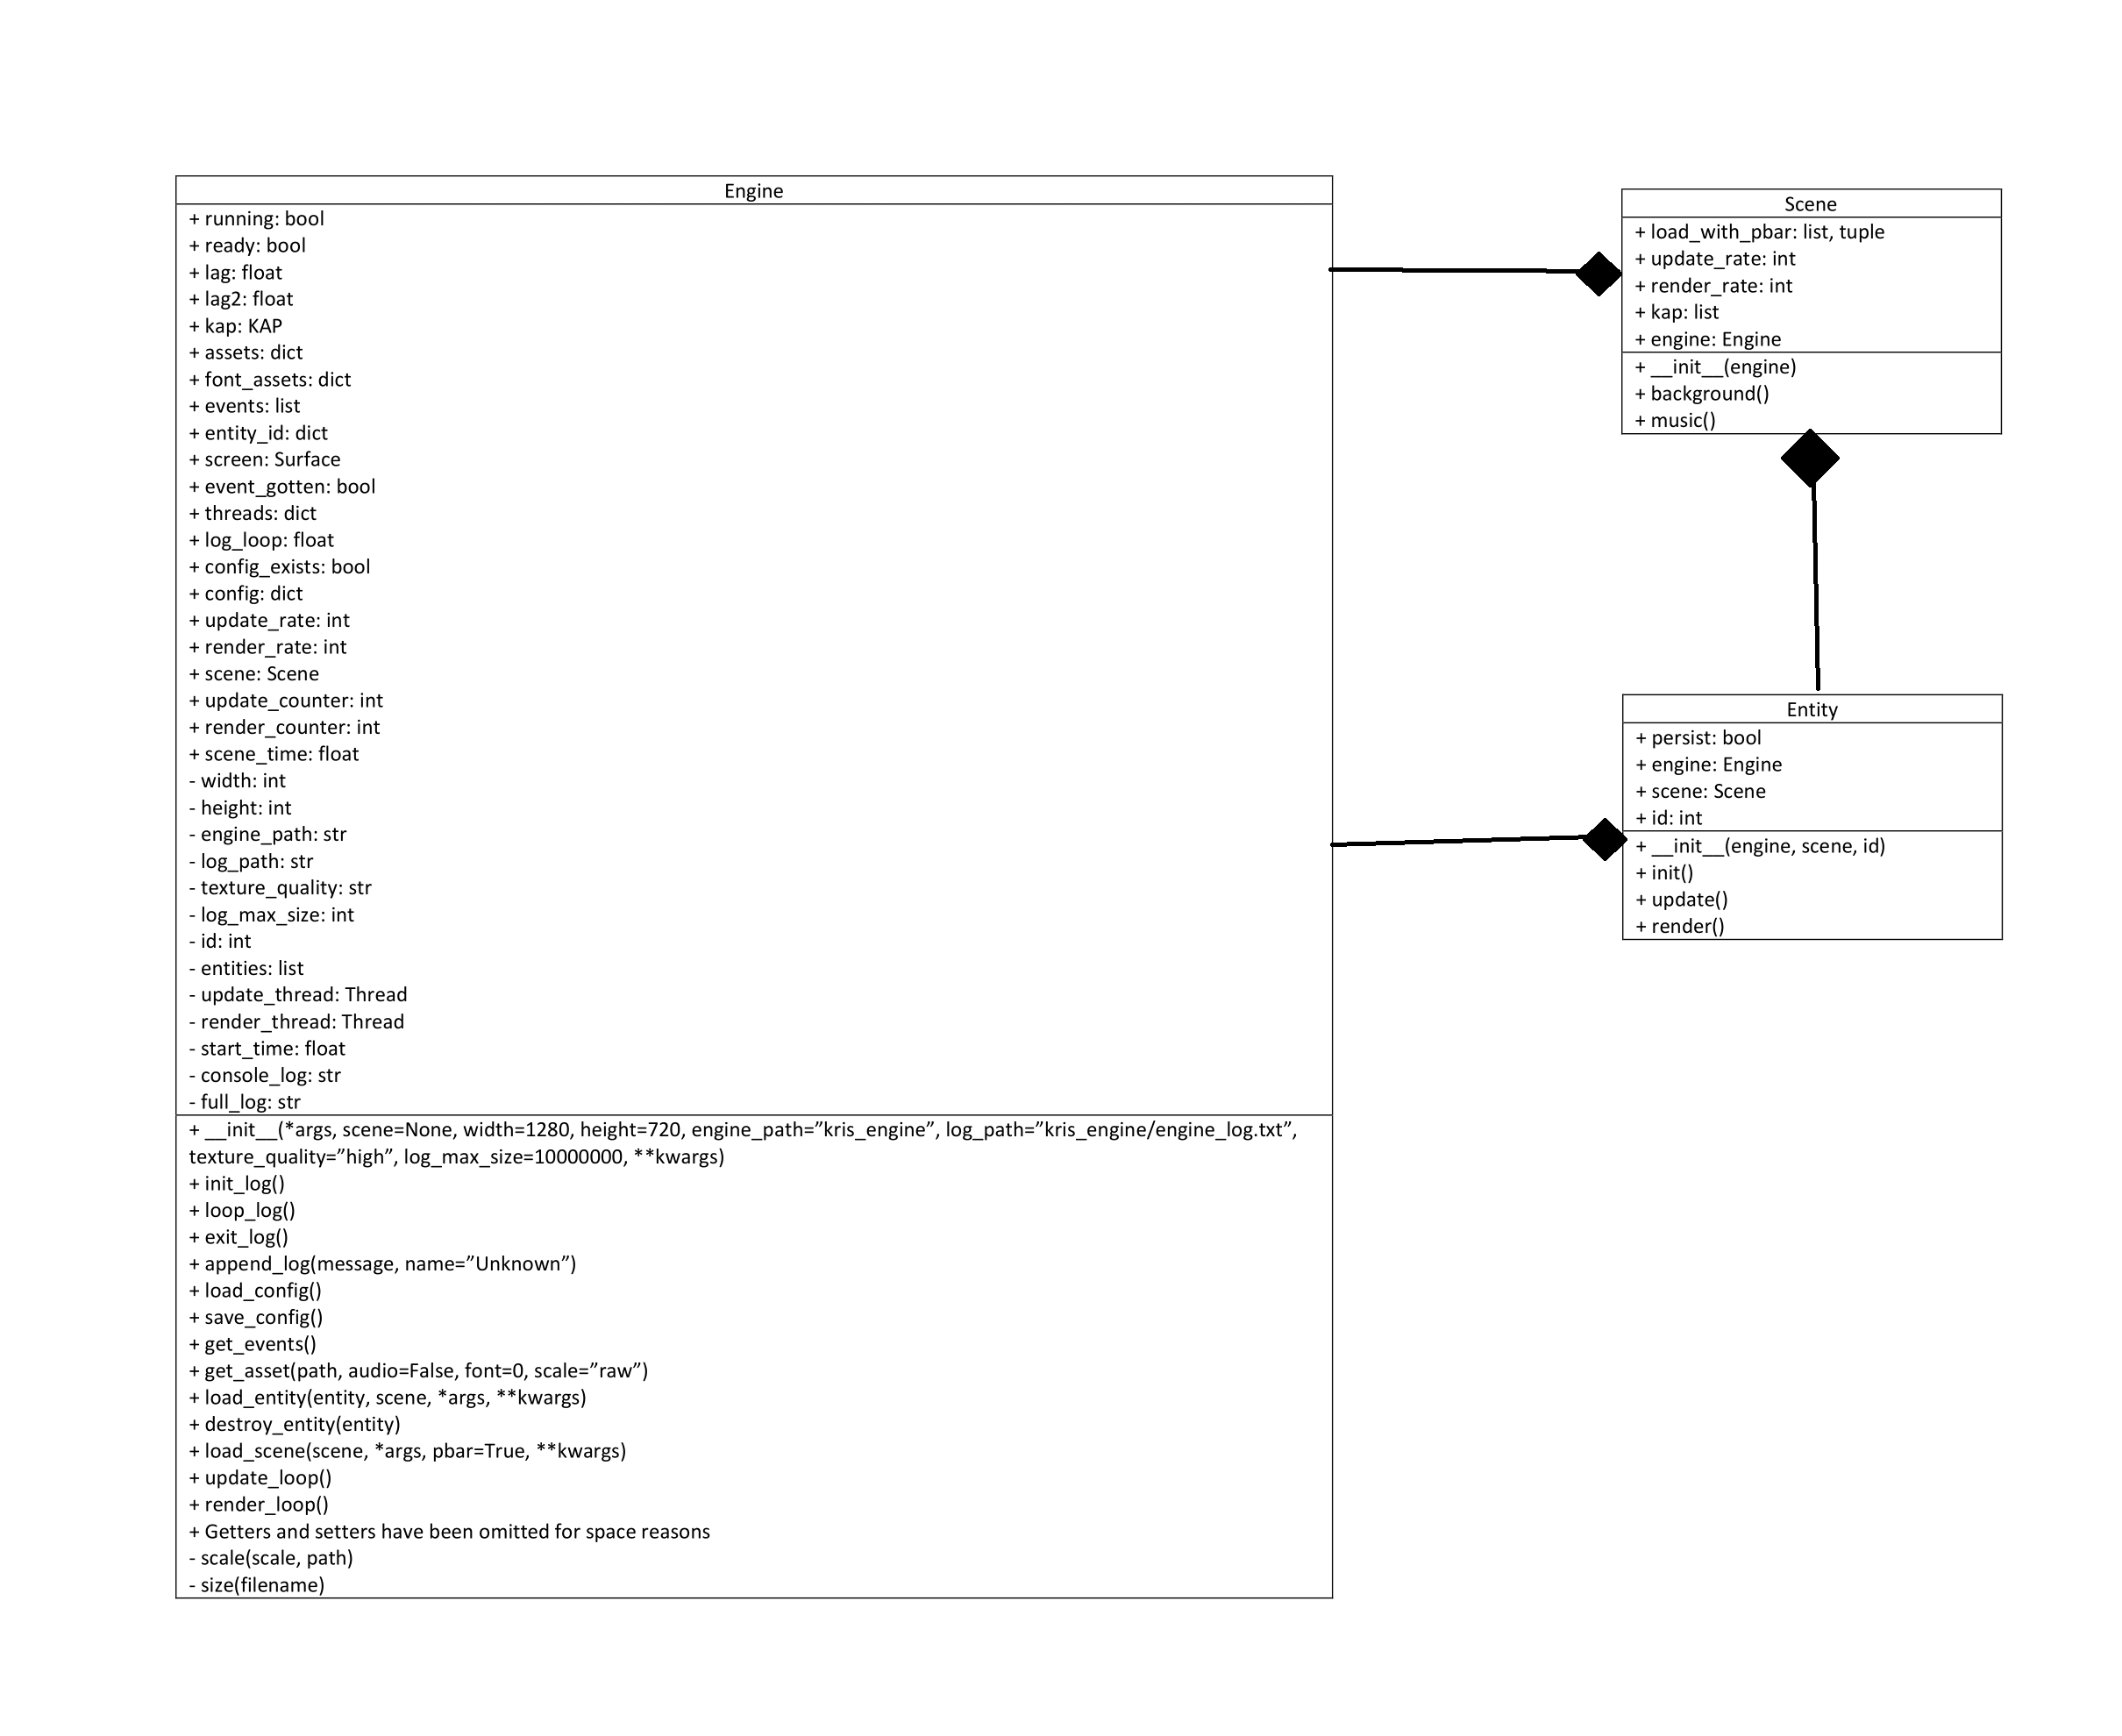
\includegraphics[width=1\textwidth]{Class diagrams-1.png}
\caption{\label{fig:class1}A class diagram of the main three engine classes}
\end{figure}

\section{Other engine scripts}

You will have seen referenced above many times the concept of KAP files. This is because of another module: kris\_engine.files. This implements a custom file type KAP which packages and compresses textures.

\subsection{files.KAP}

A wrapper for KAP files. KAP stands for Kris's Asset Package and a KAP file is designed to store many textures in a single file. It will also store different resolution copies of images for different texture qualities and compress data with a variant of run length encoding.

A KAP file is structured in two parts: a string portion and a byte portion. Some rules about the string portion:
\begin{itemize}
\item All integers are unsigned and most significant bit first
\item All strings are UTF-8
\item A 0 byte is eight bits with a value 0
\end{itemize}

The file begins with a 16-bit integer magic byte, 1993. This helps verify that we're loading the right file type. Then, an 8-bit integer representing the number of texture quality options available. Then, for as many qualities as the integer specified:
\begin{itemize}
\item string data detailing the name of the setting
\item a 0 byte
\item a non-zero 8-bit integer that the texture quality should be assigned to
\end{itemize}

Then, there's a 32-bit integer detailing how many textures there are. Each entry of the rest of the string portion is structured as follows:
\begin{itemize}
\item string data detailing the name of the file
\item 0 byte
\item 8-bit integer representing how many texture qualities the file has
\item if this byte is 0:
\begin{itemize}
    \item 64-bit integer, indicating the pointer at which the file data starts in bytes
    \item 64-bit integer, indicating the size of the file in bytes
\end{itemize}
\item if this byte is greater than 0, repeat the following for the value of the byte:
\begin{itemize}
    \item 8-bit integer corresponding to a texture quality
    \item 64-bit integer, indicating the pointer at which the file data starts in bytes
    \item 64-bit integer, indicating the size of the file in bytes
\end{itemize}
\end{itemize}
Then the corresponding files will be dumped as RLE bytes into the files at their corresponding pointers.

RLE bytes are bytes that are run length encoded. RLE bytes start with a byte that is comprised of two 4-bit integers. The first represents counter\_length, the second pattern\_length. Pattern length represents the size of chunks of data that we are processing (allowing us to compress something like 101010101010 efficiently with pattern length 2), and counter length represents the numnber of bytes allocated to storing the multiplier for a given piece of data. These are required information to encode and decode RLE bytes. Then we have to consider the excess. Take an example where we have a file with an odd number of bytes and pattern\_length 2. For the algorithm to look for patterns of length 2, we need to trim the first byte off. So, the second byte is an 8-bit integer representing the size of the excess. If this is 0, move straight on to the data, otherwise append the following number of bytes to the front of the output. Then, the rest of the bytes are in the pattern of counter\_length bytes, pattern\_length bytes. To decode, repeat the pattern\_length bytes the value of the counter\_length bytes times.

The KAP class is used as a wrapper for loading KAP files. It has the following methods:

\subsubsection{\_\_init\_\_}

This method has a positional parameter path, representing the path to the KAP file that is to be loaded. It also has an optional engine paramater, like many of the functions in the KAP class, which is used for outputting to the engine log if the engine object is passed in.

This function creates a file map, which is a dictionary that tells us which KAP file an asset comes from (the KAP class can load multiple KAP files at once). The assets dictionary is also created, containing information about the location and size of each file in a KAP file. An open dictionary is created, storing the file objects for the open KAP files, and a function is registered that closes them when the program terminates. Then the named KAP file is loaded with load\_kap.

\subsubsection{\_\_del\_\_}

Used to close all open files objects when the KAP instance is deleted or the program terminates. Takes no arguments.

\subsubsection{load\_kap}

Takes one argument, being the name of the KAP file to be loaded. Uses advanced file operation to load the KAP file, the structure of which is described above.

\subsubsection{string\_data}

A method used by load\_kap for finding where strings of unknown length terminate.

\subsubsection{load}

A method used for loading a file from a KAP file. It has a filename parameter and an optional quality parameter.

\subsection{Other files.py functions}

\subsubsection{rle\_encode}

Implements the varianets of run length encoding specified above. See the comments in the technical solution for more details.

\subsubsection{rle\_decode}

Decodes RLE bytes.

\subsubsection{rle\_brute}

Used to test multiple pattern length and counter lengths, returns the compressed file that is the smallest (and therefore most effective).

\subsubsection{build}

Uses advanced file operations, as well as Pillow for image scaling for different image qualities, to build a KAP file.

\subsection{pbar.py}

This contains a scene and entity that creates a progress bar loading screen. See comments in technical solution for more details.

\section{Classes for gameplay}

For the implementation of the classic version of exercise mode, the code was split into two script files: exercise.py, containing the ExerciseClassic scene, and gameplay.py, containing everything else.

\subsection{Grid}

Grid is an entity that manages most of the gameplay. It has a relationship of aggregation with Bean, (which is not an entity).

\subsubsection{\_\_init\_\_}

In addition to the required entity parameters, grid has one positional argument, input\_handler, which is another entity that acts like a controller. It also has many keyword arguments: rows and columns representing the size and shape of the grid, values allowing the grid to start in a non-empty state, the position of the grid and the bean queue. This method creates most of the engine attributes, sets the grid's current state to GRAVITY and loads the BeanQueue entity and Score entity, which is loaded by the grid because it needs to directly access methods and attributes of these objects. Another thing worth nothing here is that values, containing Bean objects or None (representing an empty cell), is a 1D list, not a 2D list. This is because of the fact that beans can be placed "above" the grid (above the inputed number of rows, which simply decides the square that kills you and where falling beans spawn). Increasing the size of the list is easier with a 1D list than with a 2D list.

\subsubsection{\_\_str\_\_}

Outputs the contents of the grid as a neat string. Used for debugging.

\subsubsection{update}

At any time, the grid will be in a given state. This method acts as a lookup table, executing a different update function depending on the grid's current state.

\subsubsection{update\_verify}

This method is called when updating in the VERIFY state. First we check the contents of the verify attribute, a set containing any beans that need to be removed (due to being in a colour group) this update. If there are beans that need to be removed, we first calculate the score for removing those beans, update the score counter and replace the beans with None in the grid. Our state then changes to VERIFY\_ANIMATION.

Alternatively, if there are no beans that need to be removed, we check the third cell of the top row (where beans spawn), and if it's filled then we change our state to DIE. (Death is not actually implemented, but will simply destroy the grid entity and display a message in the console). If we didn't die, then we get the next pair of falling beans from the bean queue, and calculate our score, which I will discuss now.

\subsubsection{chain\_power\_lookup, colour\_bonus\_lookup and group\_bonus\_lookup}

These are static methods that act as lookup tables for different bonuses, but it gives me an opportunity to talk about how scoring is calculated.

You will see during gameplay two numbers multipled together. The first number is equal to 10 multiplied by the maximum number number of beans popped at one time during the chain. During any point in the chain, count the number of beans that are currently being popped, and if that number is greater than the beans\_popped attribute, that becomes the new value of the beans\_popped attribute.

The second number is equal to (chain power bonus + colour bonus + group bonus). Chain power bonus is the value gotten from chain\_power\_lookup, inputting the chain power when the chain concludes. Colour bonus and group bonus are different, incrementing the bonus at each stage of the chain. At a given point during the chain, the group bonus is incremented for any group that contains more than 4 puyos. At a given point during the chain, the colour bonus is incremented if there are multiple different colours of puyo being popped at the same time. Additionally, in our score calculation, (chain power bonus + colour bonus + group bonus) must be at least 1, even if the output is 0.

\subsubsection{animate\_verify}

This method is called for updates during the VERIFY\_ANIMATION state. It increments a counter that causes actions to occur at different time periods, such as changing textures or playing a sound effect.

\subsubsection{animate\_gravity}

This method is called for updates during the GRAVITY\_ANIMATION state. The first part of this happens while there are gravity beans in the gravity attribute list. Each of these has a generator object that can be iterated through to animate the bean. When StopIteration is raised, the animation is finished, and the bean is placed in the correct position and removed from the gravity list. Additionally we also check for colour groups where this bean has fallen and correct it's texture.

When all the beans have been removed from the gravity list, then we start counting to 50 before changing to the VERIFY state. This causes a short pause beforce beginning verification again.

\subsubsection{update\_gravity\_quick}

This is an unused method that uses a quicker way of calculating where beans fall by simply removing empty cells in columns. This would be useful for replay files, but cannot be used for gameplay as since we don't know which beans have fallen we cannot animate them falling.

\subsubsection{update\_gravity}

This method is called for updates during the GRAVITY state.

For every column in the grid, we get a list containing just the contents of that column. If that column is full, we ignore it, otherwise we use the split\_list static method. This method acts exactly like the split method for a string, but for lists. It returns a 2D array, split by a separator, acting on a 1D array. This split list is very useful because the index of the list that each bean is in represents the number of rows that bean will fall. We use this information to replace these beans with gravity beans that are set to fall this distance, and replace the column with empty cells before changing state to GRAVITY\_ANIMATION.

\subsubsection{place\_bean}

Useful method for placing beans. Pads the grid if the desired position doesn't yet exist, places the bean in the grid, then checks for colour groups and updates the newly placed bean's texture.

\subsubsection{render}

At any time, the grid will be in a given state. This method first draws the beans in the grid. Then, this method acts as a lookup table, executing a different render function depending on the grid's current state. Then, we draw background3.png over the top, creating the effect of beans being behind this background.

\subsubsection{render\_grid}

Converts 1D list into 2D positions and draws the beans.

\subsubsection{render\_bean}

Accepts a bean, a row and a column as arguments. Uses pygame to draw the bean to the screen.

\subsubsection{render\_gravity}

Method executed for render calls in the GRAVITY\_ANIMATION state. Runs the render\_bean function for every gravity bean.

\subsubsection{render\_verify}

Method executed for render calls in the VERIFY\_ANIMATION state. Runs render\_bean for beans being verified, but additionally uses the counter to make them flash and be animated.

\subsubsection{render\_falling}

Method executed for render calls in the FALL state. Draws the falling bean pair by first calling render\_bean on the primary bean and then using a lookup table to find the relative position of the secondary bean dependant on rotation state.

\subsubsection{eval\_all\_textures}

Method used when passing in a pre-filled grid on initialisation. Evaluates the texture for every bean in the grid.

\subsubsection{eval\_texture}

For a given bean, checks the beans adjacent to it and updates the bean's attributes to match. Updating these attributes also updates the bean's texture.

\subsubsection{eval\_up, eval\_down, eval\_left, eval\_right}

Very similar methods used for checking the particular side of a bean, to see if a bean of the same colour, or any bean at all is present there.

\subsubsection{eval\_surrounding}

Evaluates the texture for a bean, then evalutates the texture of every bean adjacent to that beans. If you have just placed a bean, run this function to update grid textures efficiently.

\subsubsection{count\_all}

A version of count that checks for groups in the entire grid. Used when loading a non-empty grid.

\subsubsection{count}

Method for checking for groups in one part of a grid once you're placed a bean. First, check if the bean is already in the list of beans to be removed. If it isn't, then create a set containing that bean. Sets must contain unique items and will remove duplicates. Then, we use a function to get all the beans adjacent to that bean that are the same colour, and add them to a list. Then, for every bean in that list, we get the beans that are adjacent to those beans and the same colour. We keep doing this until we run out of unique beans in our list to check.  Then, if the group is larger than 4 beans, we add it to the necessary attributes.

\subsubsection{get\_surroundings}

A method for getting beans adjacent to a bean that are the same colour as that bean and also not already in the group.

\subsection{BeanQueue}

A BeanQueue is an entity that is loaded by and belongs to a Grid.

\subsubsection{\_\_init\_\_}

The only additional parameter a bean queue takes on initialisation is position, which decides where it is rendered on the screen. It has a next attribute, which is a tuple of two beans of random colours that are generated using randint from python's random module.

\subsubsection{render}

A copy of the render\_bean method from the grid, for drawing the next upcoming pair of falling beans.

\subsubsection{update}

Since I ran out of time to animate it, this entity does not have an update method.

\subsubsection{get\_next}

Returns the bean pair that was being displayed in the queue and randomly generates a new bean pair.

\subsection{Bean}

A Bean is not an entity. It is created and used by Grid.

\subsubsection{\_\_init\_\_}

A bean takes a colour as an argument on initialisation. This can either be the name of a colour, or the associated ID of that colour. It additionally has keyword arguments that allow you to get its texture.

\subsubsection{\_\_str\_\_, \_\_repr\_\_}

Debugging method that prints the bean's colour.

\subsubsection{get\_texture}

The boolean True or False of whether a bean of the same colour is adjacent to this bean on a given side can be combined into a 4-bit integer, which can be assigned to the correct texture to show in those states. Other textures require the state attribute to be set, which overrides this 4-bit integer on what texture to select.

\subsubsection{Getters and setters}

Changing a variable that would effect the texture of a bean causes it to re-evaluate it's own texture.

\subsection{GravityBean}

GravityBean is not an entity, it inherits from Bean. It is used to animate a bean falling into a new position.

\subsubsection{\_\_init\_\_}

This method has man positional arguments. bean represents the Bean object that the GravityBean is based on. destination represents the index in the grid that the bean will be placed at when it's animation is finished. row\_distance represents the number of rows that the bean will fall downwards. row and column represent the starting position of the bean.
Once these attributes have been assigned, a generator object is used to animate the falling bean. This is stored in the position attribute and should be advanced once per update.

\subsection{FallingBean}

FallingBean is not an entity and it does not inherit from anything. It contains Beans and it represents the pair of beans that the player has control over.

\subsubsection{\_\_init\_\_}

Takes the grid object as an input parameter, initialises attributes.

\subsubsection{update}

Has a counter that is incremented for timing. The texture of the primary bean is changed relative to the counter. Then we check if a rotation key is held down then we rotate. The rotation function makes it so that if a wall is in the way the bean is pushed away from the wall. Then we check if a move left or right action should occur and verify whether it is possible or if there is something in the way. If there is something in the way then moving left or right fails. We move the bean downwards relative to the counter and fall rate, fall rate is decreased if the down arrow is held. If we hit the bottom of the grid of there is a bean below when we are trying to fall, place the beans there. Otherwise, move the beans downwards. If the down arrow is held then we award points.

\chapter{Technical Solution}

\section{Features}

List operations/complex algorithms/recursive algorithms: merge sort, gameplay.py, line 909
Complex algorithm: variation of run length encoding, kris\_engine/files.py, line 152
Complex algorithm: efficient sorting of beans into colour groups, gameplay.py, line 432
Mathematical formula: score calculation, gameplay.py, line 154
Complex file operations: kris\_engine/files.py, line 281
Complex OOP: Can be seen throughout the entire project. See the documented design. Multiple classes inherit from Entity and Scene, many classes are dynamically created and composed of other classes, see Grid creating Bean objects, polymorphism is used whenever the update and render methods of an Entity are overriden... The list goes on.


\section{kris\_engine/\_\_init\_\_.py}

\inputminted[breaklines, linenos]{python}{../game/kris_engine/__init__.py}

\section{kris\_engine/files.py}

\inputminted[breaklines, linenos]{python}{../game/kris_engine/files.py}

\section{kris\_engine/pbar.py}

\inputminted[breaklines, linenos]{python}{../game/kris_engine/pbar.py}

\section{exercise.py}

\inputminted[breaklines, linenos]{python}{../game/exercise.py}

\section{gameplay.py}

\inputminted[breaklines, linenos]{python}{../game/gameplay.py}

\section{main.py}

\inputminted[breaklines, linenos]{python}{../game/main.py}

\chapter{Testing}

\href{https://youtu.be/AEm3DuqjUY8}{https://youtu.be/AEm3DuqjUY8}

In the above video, you can verify a number of tests, including:
\begin{itemize}
    \item Confirming that rotation works
    \item The falling pair is pushed away from any walls that they rotate near 
    \item The pair does not pass through any walls or other beans
    \item The pair places in the correct position and falls with gravity
    \item All the correct textures appear
    \item Scoring is correct, with footage from an emulator to prove that it produces the same values
    \item Beans fall correctly and match in groups when falling
    \item Dying is implemented correctly, no matter whether dying to an odd or even number of beans
    \item The score board displayed in the console is in the correct order
\end{itemize}

\chapter{Evaluation}

Ultimately, I greatly overestimated the scope of this project and my ability to complete it. I have successfully managed to make a working Puyo Puyo prototype, however I did not manage to create a suitable replacement to an emulated version of the game, nor even something that could be considered its equal. If I had the opportunity to complete the project again I would choose a project that was more focused on backend tasks and algorithmic complexity as these are things that I really enjoy programming, and ultimately I should stick to what I'm good at.

\end{document}